\documentclass[11pt]{article}
% Draft of the preprint (target: arXiv, mid-December 2026).  Build: pdflatex arxiv_draft.tex (twice).
% Every number is taken from results/REPLICATION_NOTES.md or the CSVs in results/; the command
% that produces each figure is `make figures`.  Passages marked [PRELIMINARY] rest on laptop runs
% (fewer cartels or seeds) and are to be replaced by the cluster runs of slurm/workshop2.sh.
\usepackage[margin=1in]{geometry}
\usepackage{amsmath,amssymb}
\usepackage{booktabs}
\usepackage{enumitem}
\usepackage{graphicx}
\usepackage[T1]{fontenc}
\usepackage[hidelinks]{hyperref}
\usepackage{caption}
\captionsetup{font=small,labelfont=bf}
\setlist{nosep,leftmargin=1.4em}
\setlist[description]{style=unboxed,leftmargin=1.2em,labelindent=0pt,itemsep=1pt}
\graphicspath{{../results/}{../results/live_2026_10/}}
\newcommand{\Fanon}{\mathcal{F}^{\mathrm{anon}}}
\newcommand{\Fid}{\mathcal{F}^{\mathrm{id}}}
\newcommand{\For}{\mathcal{F}^{\mathrm{oracle}}}
\newcommand{\LBR}{L_{\mathrm{BR}}}
\newcommand{\prelim}{\textsuperscript{[preliminary]}}

\title{Rent or Toxicity? Strategic Exploitability of Learning Market Makers\\ with Public Wallet Information}
\author{Deepu Pradeep \and Miguel Betran Menz\\ \small Massachusetts Institute of Technology}
\date{Draft, November 2026}

\begin{document}
\maketitle

\begin{abstract}
Independent learning market makers settle on spreads above the competitive level without communicating. We ask whether that profit can be attacked, by whom, with what information, and what a trading venue can do about it, on a market where every trade carries public wallet addresses. In a Glosten--Milgrom market on a price grid with closed-form benchmarks, tabular Q-learners keep 78--86\% of the gap between competitive and monopoly profit. We compute the exact best response of an entering maker to such a cartel by dynamic programming over its reaction function: it takes the entire rent in 60 of 60 cartels, and a damage-maximising variant imposes two to three times the rent at no cost to itself. The attack needs no private knowledge: an entrant that identifies the reaction function from public quotes matches the exact best response after about a thousand probing periods. Letting the cartel keep learning does not defend it. Public wallet identity is worth nothing to the entrant through wallet persistence and has value through a different channel: informed trading comes in spells, and who just traded reveals the spell before prices do. On Hyperliquid data we find the same mechanism at work: the makers who earn the spread take two to four times fewer fills from wallets that were toxic in the past, every day and every hour of a four-week recording. When the price grid pins the spread at one tick, rent can only come from which fills a maker gets; venue rules (anonymity, a priority fee, a request allowance) and the makers' own defences move the toxic flow between participants, and none of them protects the rent.
\end{abstract}

\section{Introduction}

An \emph{exchange} is a venue where buyers and sellers of an asset meet. \emph{Market makers} post standing offers to buy and to sell; \emph{takers} accept them. The difference between a maker's buying and selling price, the \emph{spread}, is the price takers pay for trading at once. With enough competing makers, undercutting drives the spread down to the \emph{competitive} level, where a maker's gains from ordinary takers just cover its losses to better-informed ones. A recent literature shows that learning algorithms do not get there: independent reinforcement learners in a pricing game settle on higher prices and sustain them with learned punishments \cite{calvano}, and the same happens to learning market makers \cite{cfl,cont}. What they earn above the competitive level is a \emph{rent}: profit that exists only because the makers refrain from undercutting one another.

That this coordination arises is documented. Whether it can be \emph{attacked} is not: how much of the rent an adversary can take, what the adversary needs to know, whether the learners can defend themselves, and what the venue's rules change. These are security questions about a learned multi-agent equilibrium, and they have a specific difficulty in a market: a wide spread is also the correct charge for trading against informed takers. Rent and \emph{toxicity} (a high share of informed flow) look identical in the record of trades, so an adversary who undercuts a wide spread may be taking a rent or walking into losses.

We study this as a security game. The \emph{defenders} are learning makers, the \emph{adversary} is a maker who enters a trained population, \emph{nature} is the flow of takers, and the \emph{designer} is the venue, which chooses the price grid, what is public, and how orders at the same price are served. Hyperliquid, an exchange whose matching runs on a public blockchain, is our laboratory, for one reason: every order and trade there carries a persistent public account address (a \emph{wallet}), so what an adversary may know about who is trading is a design choice of the venue rather than a constant, and its consequences can be measured on the public record.

\paragraph{Contributions.}
\begin{enumerate}
\item \textbf{Exploitability of learned rent, exactly.} A cartel whose learning has stopped is a deterministic reaction function, so the entrant's problem is a finite Markov decision process that backward induction solves exactly. The exact best response takes the whole rent in 60 of 60 cartels; the hand-written undercutting rules used in earlier work reach 55--70\% of it. The damage-maximising entrant imposes two to three times the rent while earning nothing and risking nothing (\S\ref{sec:rq2}).
\item \textbf{The attack is public.} Every value of the reaction function appears on the public book. An entrant that records it cell by cell and solves the estimate matches the exact best response after about 1000 probing periods, for two and for three incumbents. Re-learning by the cartel buys back half of what a stale attacker takes and nothing against one that re-solves (\S\ref{sec:rq2}).
\item \textbf{What identity is worth, and why.} We price the entrant's information as the difference between nested information sets. The mechanism the first intuition suggests (a toxic wallet trades again) is worth zero at the persistence the data show. Value comes from spells of informed trading combined with the delay before a trade's outcome is knowable: a known wallet's trade reveals the spell at once (\S\ref{sec:rq1}).
\item \textbf{The mechanism on a real book.} On four weeks of Hyperliquid data with wallets on every trade, the quoted spread on the major markets is one price step almost always, so makers cannot compete on price; the ten most active makers nonetheless earn where others lose, and they do it by taking two to four times fewer trades from wallets classified as toxic on earlier days (\S\ref{sec:data}).
\item \textbf{Defences on one frontier.} With the spread pinned, we model the queue of standing orders and compare the venue's rules and the makers' own defences by what the defenders earn alone and under the worst attacker, together with what ordinary takers get. No lever protects the rent; they decide who holds the toxic flow (\S\ref{sec:rq3}).
\end{enumerate}

\section{Related work}

\paragraph{Algorithmic collusion.} Calvano et al.\ \cite{calvano} showed that independent Q-learners in a repeated pricing game converge to supra-competitive prices sustained by learned punishment. Colliard, Foucault and Lovo \cite{cfl} and Cont and Xiong \cite{cont} carry this to market making in the Glosten--Milgrom model \cite{gm}, a dealer facing informed and uninformed takers, where the wide quote has a second reading as the price of adverse selection. Cartea, Chang and Penalva \cite{ccp} show that the price grid itself sustains supra-competitive quotes, and Dou, Goldstein and Ji \cite{dgj} study AI traders colluding through price impact. We take the environment and the learners from \cite{cfl} and the test of the mechanism from \cite{calvano}; our question starts where theirs ends.

\paragraph{Adversaries of learners.} Deng, Schneider and Sivan \cite{dss} characterise what an optimiser can earn against a no-regret learner: at least its Stackelberg value (what it would earn by committing to an action first), and strictly more against the common mean-based learners. Brown and MacKay \cite{brownmackay} study a fast pricing algorithm steering a slower one. Gleave et al.\ \cite{gleave} show that a frozen reinforcement-learning policy is exploitable by driving it into states it never trained on. McMahan et al.\ \cite{mcmahan} and Lanctot et al.\ \cite{psro} give the double-oracle loop, in which each side in turn best-responds to the other's current policies. We compute the attacker's side exactly rather than learning it, and we place every result against the Stackelberg value.

\paragraph{Identity and data.} Zhai \cite{zhai} documents on Hyperliquid that public trader identity predicts adverse selection and returns; we turn that observation into an information set and price it. Albers et al.\ \cite{albers} publish the order-level archive we use alongside our own recorder. The practitioner template for market making is Avellaneda and Stoikov \cite{as}.

\section{Definitions and notation}\label{sec:definitions}

We define each market term once, in the language of games and control. Appendix~\ref{app:glossary} is the complete list.

A maker's \emph{quote} is a standing offer to sell above and to buy below a public reference price, the \emph{mid} $m_t$. Prices live on a grid whose step is the \emph{tick} $\theta$; a maker's action is its \emph{half-spread} $h\in\{1,\dots,K\}$ in ticks. The lowest half-spread among the makers is the \emph{best quote}. A \emph{fill} is an accepted offer; the public record of fills is the \emph{tape}. A maker's payoff on a fill is the difference between its price and the asset's value $V_t$. A taker is \emph{informed} if she knows $V_t$ and trades only when the maker loses, and \emph{uninformed} otherwise; being matched with the informed kind is \emph{adverse selection}, and the \emph{toxicity} $\alpha$ of a flow is its informed share. The \emph{mark} of a fill is the value against which its profit is scored; on real data it is the mid some seconds later and the profit so measured is the \emph{markout}.

A trained set of makers that sustains a wide spread is a \emph{cartel} (no communication is implied). Its \emph{reaction function} is the map from last period's quotes to its next quotes. The \emph{entrant} is one additional maker; to \emph{undercut} is to quote inside the best incumbent quote. The entrant's \emph{information set} is what it may condition on: $\Fanon$ (the tape without wallets) $\subset\Fid$ (the tape with wallets) $\subset\For$ (plus the hidden state of the taker flow).

\section{Model}\label{sec:model}

\paragraph{One period.} $N$ incumbents and possibly one entrant commit half-spreads simultaneously. Nature draws the value $V_t=m_t\pm d_t$, $d_t\sim\mathrm{Exp}(\mu)$, and one taker. An informed taker trades if and only if the best quote is strictly inside $V_t$; an uninformed one trades if and only if a private valuation $m_t+\mathcal N(0,\sigma_L^2)$ crosses the best quote. One unit goes to a maker at the best quote (ties split at random). The fill becomes public; its mark becomes public $L$ periods later (the \emph{mark lag}). The value is redrawn every period, which makes the game stationary and its benchmarks closed-form. We use $K=24$, $\theta=0.5$, $\sigma_L=8$, $\mu=5$, episodes of $T=100$ periods.

\paragraph{Benchmarks.} When the best quote is $h$ and the informed share is $\alpha$, the market-wide expected payoff per period is
\[
\Pi(h;\alpha)=(1-\alpha)\,2x\,\bar\Phi(x/\sigma_L)-\alpha\,\mu\,e^{-x/\mu},\qquad x=h\theta ,
\]
with $\bar\Phi$ the standard normal tail probability. The makers at the best quote split it. The \emph{break-even quote} $h^C=\min\{h:\Pi\ge0\}$ is the Nash point of the one-shot game, since any wider quote is profitably undercut; $h^M=\arg\max_h\Pi$ is the joint monopoly. At $\bar\alpha=0.1,0.3,0.5$ these are $(h^C,h^M)=(2,13),(4,14),(8,17)$ and $\Pi^M-\Pi^C=1.90,1.38,0.66$. Because the informed loss never vanishes at any quote, no quote is immune to informed flow.

\paragraph{Outcome measures.} Let $\Pi_{\mathrm{nominal}}$ be the frozen incumbents' payoff per period when they play alone. The \emph{rent index} $C=(\Pi_{\mathrm{nominal}}-\Pi^C)/(\Pi^M-\Pi^C)$ places them between Nash (0) and monopoly (1). With adversary $A$ present they earn $J(A)$; their \emph{best-response loss} is $\LBR^A=\Pi_{\mathrm{nominal}}-J(A)$ and the \emph{fraction of rent destroyed} is $\kappa_A=\LBR^A/(\Pi_{\mathrm{nominal}}-\Pi^C)$. \emph{Rent units} divide any payoff by $\Pi^M-\Pi^C$. The game is general-sum, so the defenders' loss and the adversary's gain are reported separately. For takers we report the uninformed taker's expected gain from trade, which is also closed-form: $S(h;\alpha)=(1-\alpha)\,2\,[\sigma_L\phi(x/\sigma_L)-x\bar\Phi(x/\sigma_L)]$, decreasing in the best quote.

\paragraph{Learners.} Incumbents are tabular Q-learners as in \cite{cfl}: state (own last quote, best rival's last quote), $\epsilon$-greedy exploration with exponential decay, discount $0.95$, $2\times10^4$ training episodes. At evaluation they are \emph{frozen}: greedy play, no updates. All treatments in a cell share random draws.

\paragraph{Taker flow.} Takers come from a population of $M=50$ wallets with persistent types $\alpha_j$ (stratified quantiles of a Beta distribution with mean $\bar\alpha$ and concentration $\kappa_\alpha$). A hidden \emph{regime} $z_t\in\{\text{calm},\text{toxic}\}$ is kept with probability $\rho_z$ and otherwise redrawn so that the mean toxicity stays $\bar\alpha$. In the toxic regime wallet $j$ arrives with weight proportional to $\alpha_j$, in the calm one to $1-\alpha_j$; at $\kappa_\alpha=1$ and $\bar\alpha=0.3$ the two regimes have toxicity $0.65$ and $0.15$. Who just traded is therefore evidence about the state the next taker shares. Each piece is there because the data asked for it (\S\ref{sec:data}): the same wallet rarely trades twice in a row, informed trading clusters in time, and a fill's outcome is knowable only after the price has moved.

\paragraph{Two modes of one environment.} In the \emph{spread mode} makers choose $h$. In the \emph{queue mode} the spread is pinned at one value and each maker chooses to \textsc{rest} (keep a standing order at the best price) or stay \textsc{out}; resting makers are served first-in-first-out, a filled maker rejoins at the back, and a maker that steps out loses its place. The queue mode exists because on the real book the spread does not move (\S\ref{sec:data}).

\section{Rent and its exploitability}\label{sec:rq2}

\paragraph{Learners coordinate above the Nash point.} Two or three Q-learners settle at $10.8$, $14.9$, $17.4$ ticks at $\bar\alpha=0.1,0.3,0.5$, against Nash quotes $2,4,8$ and monopoly quotes $13,14,17$: $C=0.83,0.86,0.78$ (standard deviation over ten seeds $0.01$--$0.02$), replicating \cite{cfl}. A grid over $N\in\{2,3,5\}$, learning rate and initialisation gives $C=0.71$--$0.87$ throughout. The mechanism is \emph{restraint}: in 55--83\% of visited states a rival sits at or inside the monopoly quote, so undercutting would pay this period, and in 96--100\% of those states the learner's greedy action forgoes the undercut. The rent needs the learners' memory: two stateless no-regret learners (EXP3 over quotes) earn $C\in[-0.16,+0.12]$ at every toxicity and learning rate, while a single one finds the monopoly quote.

\paragraph{Rule adversaries.} Against 180 frozen cartels with $C\in[0.42,0.97]$, three entrant rules (undercut by one tick; undercut only while own fills indicate the spread exceeds the break-even; the same with the true toxicity) destroy a fraction $\kappa_A=0.71$--$0.73$ of the rent, flat in $C$. More collusive cartels lose more in absolute terms only because they have more to lose.

\paragraph{The exact best response.} A frozen cartel answers last period's quote vector deterministically, the entrant's own quote is part of that vector, and one-period rewards are $\Pi$ split among the makers at the best quote. The entrant therefore faces a finite-horizon Markov decision process with $K^{N+1}$ states and deterministic transitions, which backward induction solves exactly for any objective $\lambda\,(\text{own profit})-(1-\lambda)\,(\text{incumbents' profit})$. Simulated and computed values agree to $0.02$. Results over 60 cartels (Figure~\ref{fig:br}):
\begin{itemize}
\item The profit-maximiser ($\lambda=1$) takes everything: $\LBR>C$ in 60 of 60 cartels, $\kappa_A=1.14$--$1.29$, and the entrant earns $1.08$--$1.20$ rent units, the monopoly profit itself. The rules reach 55--70\% of that. The Stackelberg value of the stage game, what the entrant could earn by committing against rational incumbents, is $0.06$ on the same cartels: almost all of the take is exploitation of the learned dynamics.
\item It undercuts the \emph{reaction}, not the last fill: it quotes one tick inside what the incumbents are about to quote in 100\% of periods, and holds the cartel in states it never visits alone (86--99\% of periods), where the learned response sends it wider ($10.8\to15.9$ ticks at $\bar\alpha=0.1$).
\item The damage-maximiser ($\lambda=0$) steers the cartel \emph{tight}, to 4--7 ticks, inside its break-even, by quoting above it. It takes no fills, earns nothing and risks nothing, and the incumbents absorb toxic flow at losing quotes: $\LBR=1.3$ at $\bar\alpha=0.3$ and $2.7$--$2.8$ at $0.5$, two to three times the rent.
\end{itemize}

\begin{figure}[t]\centering
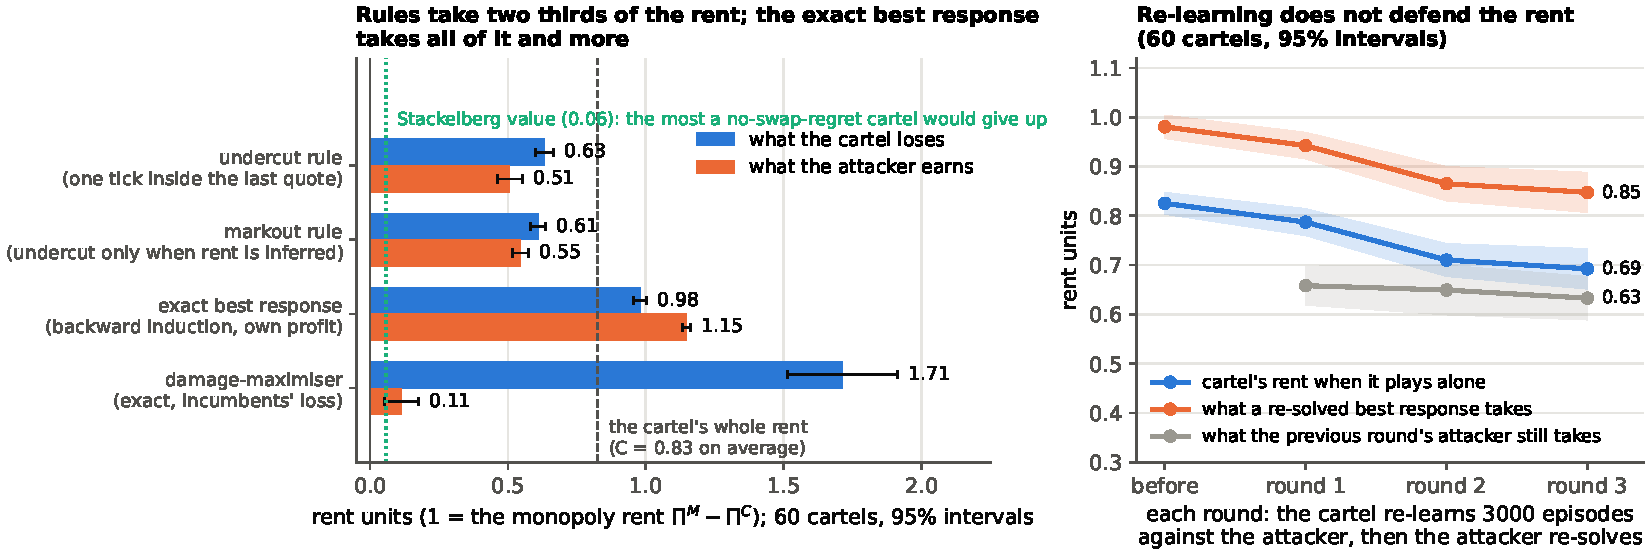
\includegraphics[width=0.86\textwidth]{fig_attackers.pdf}
\caption{Left: what each adversary takes from a frozen cartel (the cartel's loss and the adversary's own profit, rent units; means over 60 cartels, 95\% intervals); the dashed line is the cartel's entire rent. Right: the double oracle by round.}\label{fig:br}
\end{figure}

\paragraph{The attacker with public information only.} The exact best response uses the cartel's Q-tables. It does not need them. Each period the public book shows every incumbent's new quote next to the pair (own last quote, best rival's last quote) it answered, and the entrant sets the rival's quote whenever its own is the tightest. The entrant records the reaction function cell by cell, treats unseen cells as ``the incumbent goes to $h^C$'' so that the plan never relies on them, and solves the same decision process on the estimate. With a probing budget of $B$ periods of random quotes (Table~\ref{tab:public}, Figure~\ref{fig:public}), two episodes are enough to take the rent and ten to match the oracle to the second decimal, for $N=2$ and $N=3$ alike: the best response's own path uses 20--40 of the cells, and random quoting reaches them quickly. Probing has a cost (random quotes earn nothing), so the best budget is short.

\begin{table}[t]\centering\small
\begin{tabular}{lccc}
\toprule
probing budget $B$ (periods) & $N=2$ ($\bar\alpha=0.1$ / $0.3$ / $0.5$) & $N=3$ ($0.1$ / $0.3$ / $0.5$) & path identified \\
\midrule
oracle (true tables) & 1.21 / 1.09 / 1.17 & 1.20 / 1.08 / 1.16 & 1 \\
0 & 0.21 / 0.09 / 0.18 & 0.22 / 0.09 / 0.21 & .09--.23 \\
200 & 1.12 / 1.06 / 1.15 & 1.10 / 1.07 / 1.14 & .53--.75 \\
1000 & 1.20 / 1.08 / 1.16 & 1.20 / 1.09 / 1.16 & .92--1.00 \\
5000 & 1.21 / 1.09 / 1.16 & 1.21 / 1.09 / 1.16 & 1.00 \\
\bottomrule
\end{tabular}
\caption{The public-information attacker: entrant's profit after probing, rent units, 60 frozen cartels. ``Path identified'': the share of the reaction-function cells on the exact best response's path that the attacker has observed.}\label{tab:public}
\end{table}

\begin{figure}[t]\centering
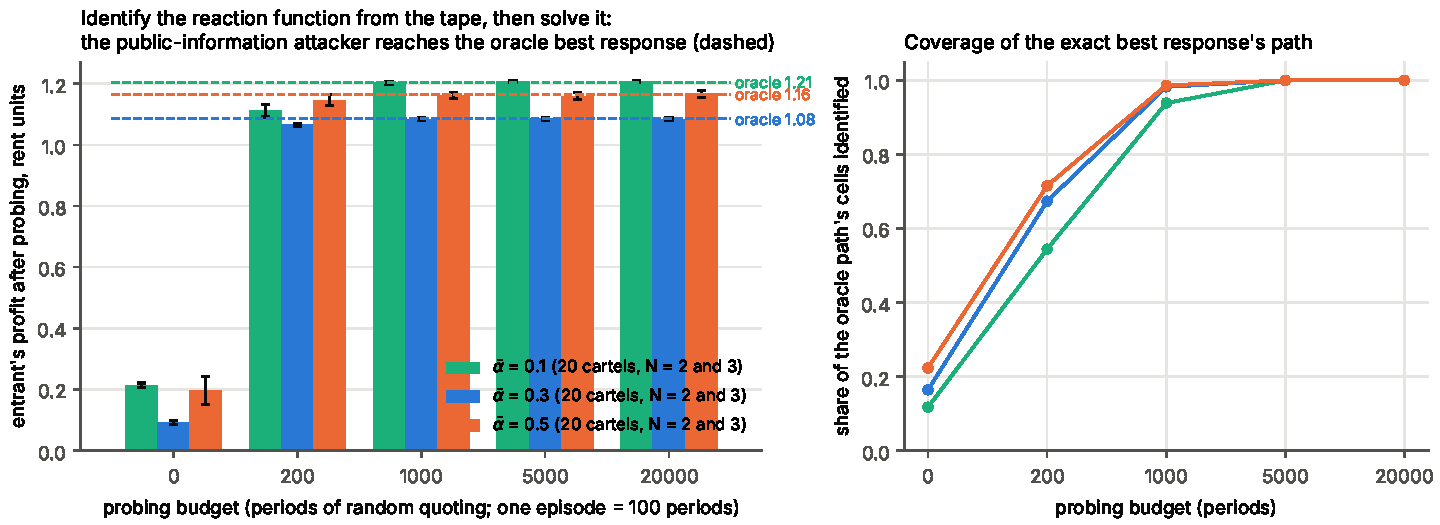
\includegraphics[width=0.8\textwidth]{fig_public_attacker.pdf}
\caption{The public-information attacker against the probing budget.}\label{fig:public}
\end{figure}

\paragraph{A cartel that keeps learning.} A frozen cartel is the easy case for identification. We let the cartel resume Q-learning under attack for 3000 episodes, with fresh exploration, and compare four entrants (Figure~\ref{fig:relearn}; 15 two-maker cartels, five per $\bar\alpha$, laptop run). While the cartel learns, an oracle that re-solves from its current Q-tables earns $0.45$--$0.64$ rent units instead of $1.1$, because the exploring cartel quotes tighter and there is less to take; the public-information attacker earns $0.40$--$0.60$, within $0.05$ of the oracle throughout, and $1.12$ against $1.13$ once the cartel stops. The cartel's own profit is at or slightly below the Nash level for the whole period ($-0.09$ to $-0.01$ rent units relative to it): learning under attack destroys the rent and does not defend it. Forgetting old observations, the natural design against a drifting target, lowers the attacker's profit by $0.01$--$0.06$ while the cartel learns and by $0.05$--$0.08$ once it stops: the reaction function drifts slowly enough that an old observation is worth more than none. The only attacker the cartel recovers against is a stale one that never re-solves (the cartel keeps $0.05$--$0.13$).

\begin{figure}[t]\centering
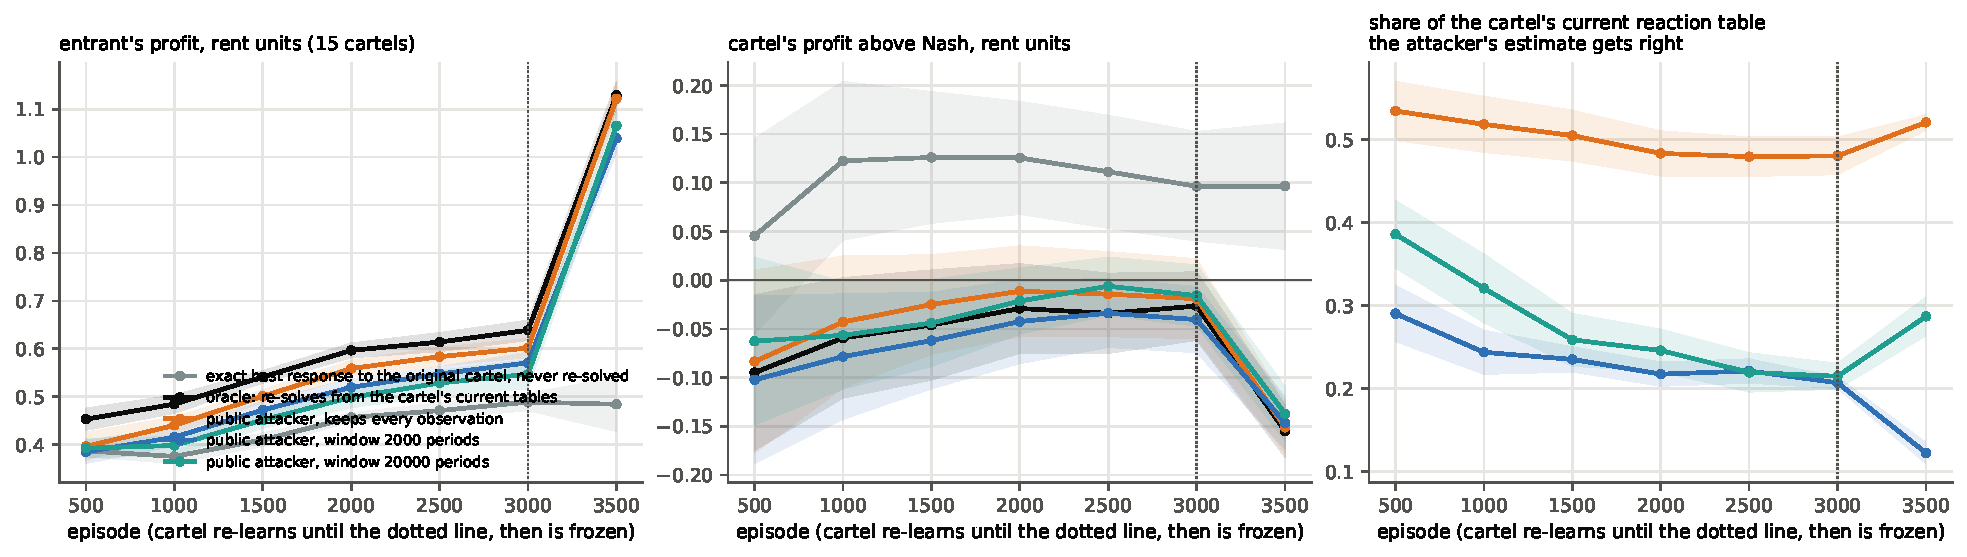
\includegraphics[width=\textwidth]{fig_relearn_attack.pdf}
\caption{Attackers against a cartel that re-learns until the dotted line and is then frozen. Bands: 95\% intervals over cartels.}\label{fig:relearn}
\end{figure}

\paragraph{Does learning defend the cartel? The double oracle.} The cartel resumes learning against the fixed best response, is frozen again, and the entrant re-solves; this is repeated. In three rounds on 60 cartels, re-learning buys back half of what the now-stale attacker takes (its profit falls from $1.2$ to $0.5$) and nothing against the re-solved one ($\LBR\ge0.9\,C$ in every cartel and round), while the cartel's own rent erodes from $0.83$ to $0.69$.

\paragraph{Running the loop long.}\prelim{} Three rounds might be too few for the cartel to find a defence. We run six, in two modes: the cartel re-learns against the latest best response, or against a uniform mixture of every best response found so far (an adversarially trained cartel). On the first cartels of an ongoing run (four and three, $\bar\alpha=0.1$; Figure~\ref{fig:psro}) the loop does not settle anywhere better for the cartel: its loss to the re-solved best response equals its rent plus $0.21$ in every round and both modes, the best response earns $1.18$--$1.19$ every time, and the rent wanders between $0.62$ and $0.86$ without trend. Training against the mixture buys robustness to the attackers trained against (the previous round's attacker falls to $0.38$) and nothing against a new one. The public-information attacker equals the oracle in every round, so the realistic entrant is the one in the loop. Adversarial training makes the cartel neither less exploitable nor reliably less collusive.

\begin{figure}[t]\centering
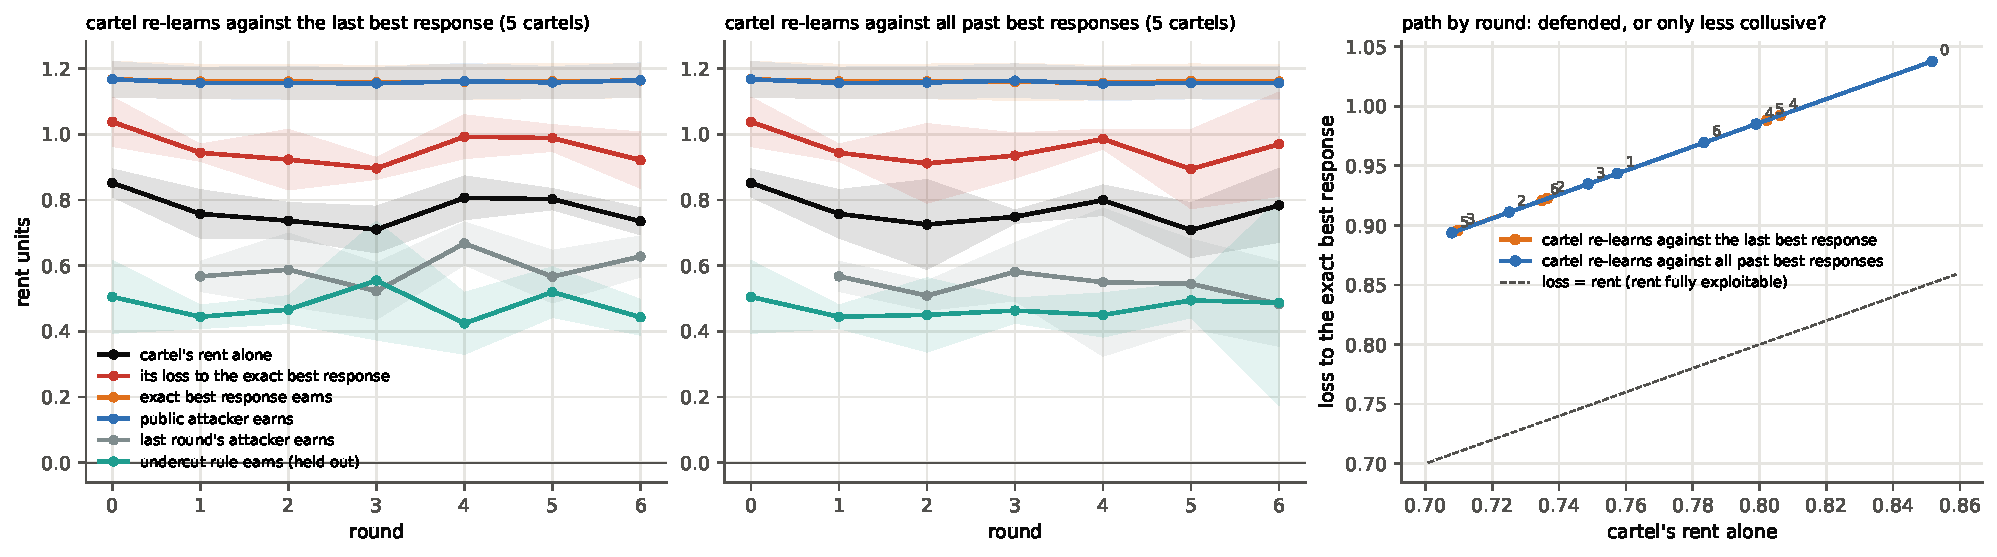
\includegraphics[width=\textwidth]{fig_psro.pdf}
\caption{The double oracle over six rounds, by what the cartel re-learns against, and the path of (rent, loss to the exact best response) by round.}\label{fig:psro}
\end{figure}

\paragraph{No-regret learners.} The same holds for a different class of learner. A single EXP3 learner over quotes, still learning throughout the attack, finds the monopoly quote alone ($C=0.89$--$0.98$) and is then taken for four to eight times its Stackelberg value by the one-tick undercut rule, losing its whole rent ($1.00$--$1.15$ rent units) at every learning rate: the mean-based learner moves slowly toward tighter quotes and the rule follows one tick inside. This is the ``strictly more than Stackelberg'' case of \cite{dss}, observed.

\paragraph{Robustness.} Cartels keep $C=0.80$--$0.86$ and $\kappa_A=0.65$--$0.75$ against the rules on any market calmer than their training one; on a more toxic one their rent collapses ($C=0.23$ for the $\bar\alpha=0.1$ cartel at $0.5$).

\section{Information: what wallet identity is worth}\label{sec:rq1}

The entrant on $\Fid$ runs a Bayesian filter: posteriors over wallet types from scored fills and a belief over the regime from the sequence of wallets. It acts on its forecast of the next taker's toxicity, undercutting when the incumbents' quote exceeds the break-even for that forecast and standing back otherwise. On $\Fanon$ the same filter sees only outcomes, which arrive $L$ periods late. Identity's value is the first entrant's profit minus the second's, paired by seed (Figure~\ref{fig:lag}).

\begin{itemize}
\item \textbf{Persistence is not the mechanism.} If the wallet that just traded trades again next with probability $\rho$, identity is worth $+0.15$ to $+0.30$ rent units at $\rho=0.9$--$0.99$ and exactly zero at $\rho=0$. On Hyperliquid the same wallet trades again next 2--5\% of the time.
\item \textbf{Spells plus a mark lag are.} With regimes and an immediate mark ($L=1$), identity adds only $+0.03$ to $+0.06$: the last fill's outcome is as good a signal of the regime as its author. As the mark arrives later the anonymous entrant's profit falls and the identity entrant's does not; the increment grows from $+0.06$ to $+0.16$ ($\pm0.07$) at $\bar\alpha=0.5$, $\rho_z=0.99$, and peaks where the lag equals the regime's lifetime.
\item \textbf{It is zero where an undercut pays in every state} ($\bar\alpha\le0.3$ against wide cartels), and it can hurt: at low type dispersion the incumbents' reaction punishes the identity entrant's moving quote in three of ten cartels. The reaction function is part of the game.
\end{itemize}

\begin{figure}[t]\centering
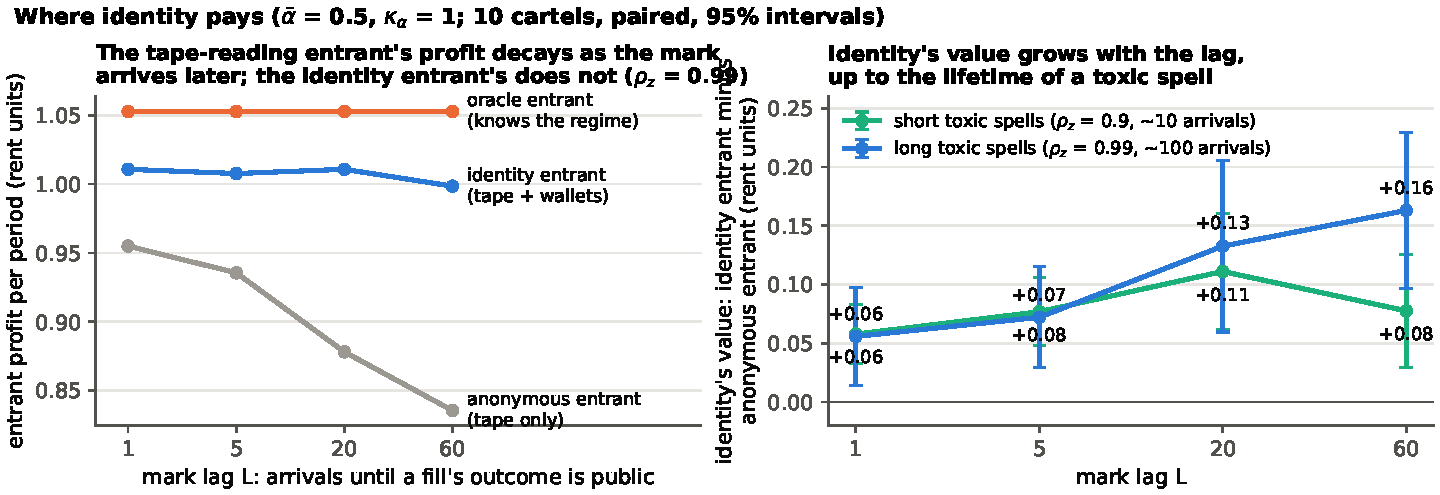
\includegraphics[width=0.7\textwidth]{fig_lag.pdf}
\caption{The anonymous entrant's profit decays with the mark lag; the identity entrant's does not.}\label{fig:lag}
\end{figure}

\section{Evidence from Hyperliquid}\label{sec:data}

We use the public order-level archive \cite{albers} and our own recorder of trades (with both wallets) and of the best bid and ask, covering October 6 to November 1, 2026, continuous from October 25, on BTC, ETH, SOL and HYPE. A maker's markout at ten seconds is its profit on the fill against the mid ten seconds later, in basis points (bps, hundredths of a percent) of the price.

\paragraph{The price cannot move.} The quoted spread on BTC, ETH and SOL is one tick essentially always (its 90th percentile equals its median). A fill at the best price pays that tick and then loses $0.2$--$0.4$ bps to the mid within ten seconds on every coin. On such a book rent cannot live in the spread.

\paragraph{Someone still earns.} Classifying wallets as makers by their activity, the ten most active earn $0.3$--$1.0$ bps per fill more than everyone else at the same price, and their ranking persists from day to day (rank correlation of daily markouts with the previous day's $0.5$--$0.9$).

\paragraph{How: by who is on the other side.} We type every taker wallet on the data before October 12 by the markouts it inflicted (benign and toxic thirds) and score everything from October 20 on: $1.44$M, $0.85$M, $0.38$M and $1.49$M later fills at the best price on the four coins. The top-10 makers take $0.14/0.35/0.43/0.30$ of the benign wallets' fills against $0.04/0.12/0.17/0.16$ of the toxic wallets' (ratios $3.6/2.8/2.5/1.9$). The gap is positive and more than two standard errors wide on 33 of 35 coin-days and in 94 of 96 coin-hours; it holds on fills after which the mid did not move within a second, which speed alone cannot explain; and labels stay valid: typing on day $d$ and scoring on day $d+k$ gives a flat gap out to $k=10$ (Figures~\ref{fig:idsel},~\ref{fig:long}). Recent volatility adds a small effect on two coins (a 20\% relative drop in the top makers' share on ETH and HYPE). The wallets who earn the spread are the ones who avoid the wallets that were toxic in the past. A toxic label is a durable attribute of a wallet across days even though the same wallet rarely trades twice in a row.

\begin{figure}[t]\centering
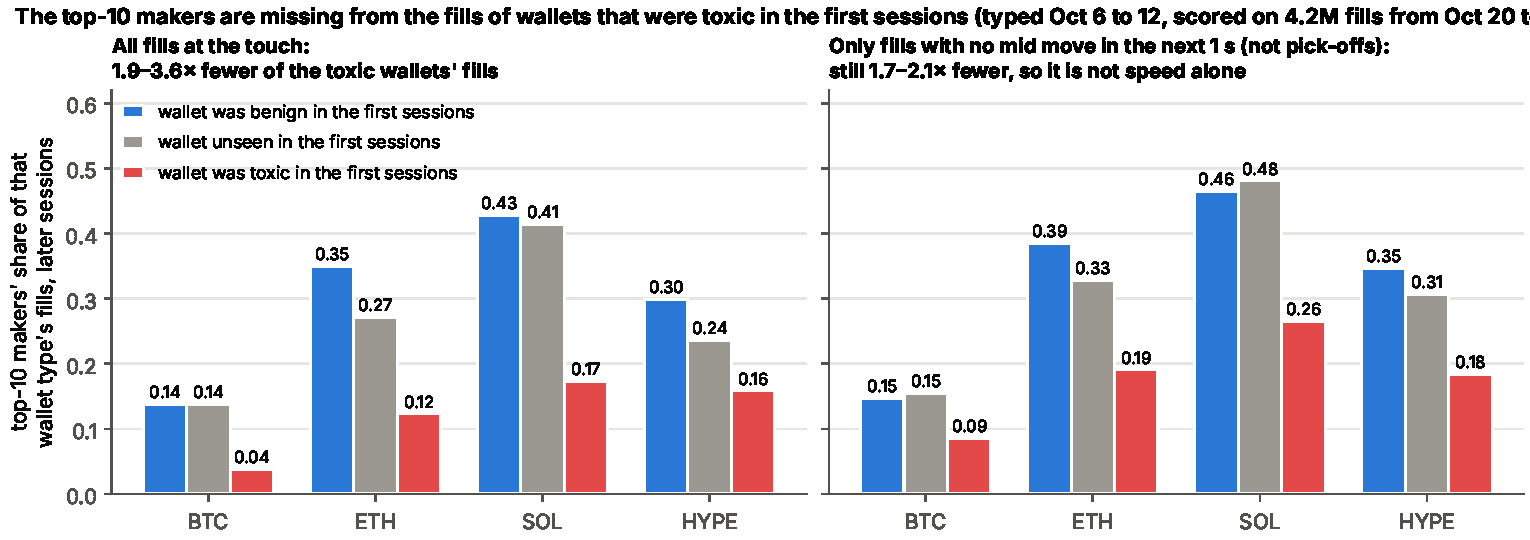
\includegraphics[width=0.74\textwidth]{fig_identity_selection.pdf}
\caption{Identity selection on the book: the top-10 makers' share of fills at the best price, by the taker wallet's earlier type. Right: only fills after which the mid did not move within one second.}\label{fig:idsel}
\end{figure}
\begin{figure}[t]\centering
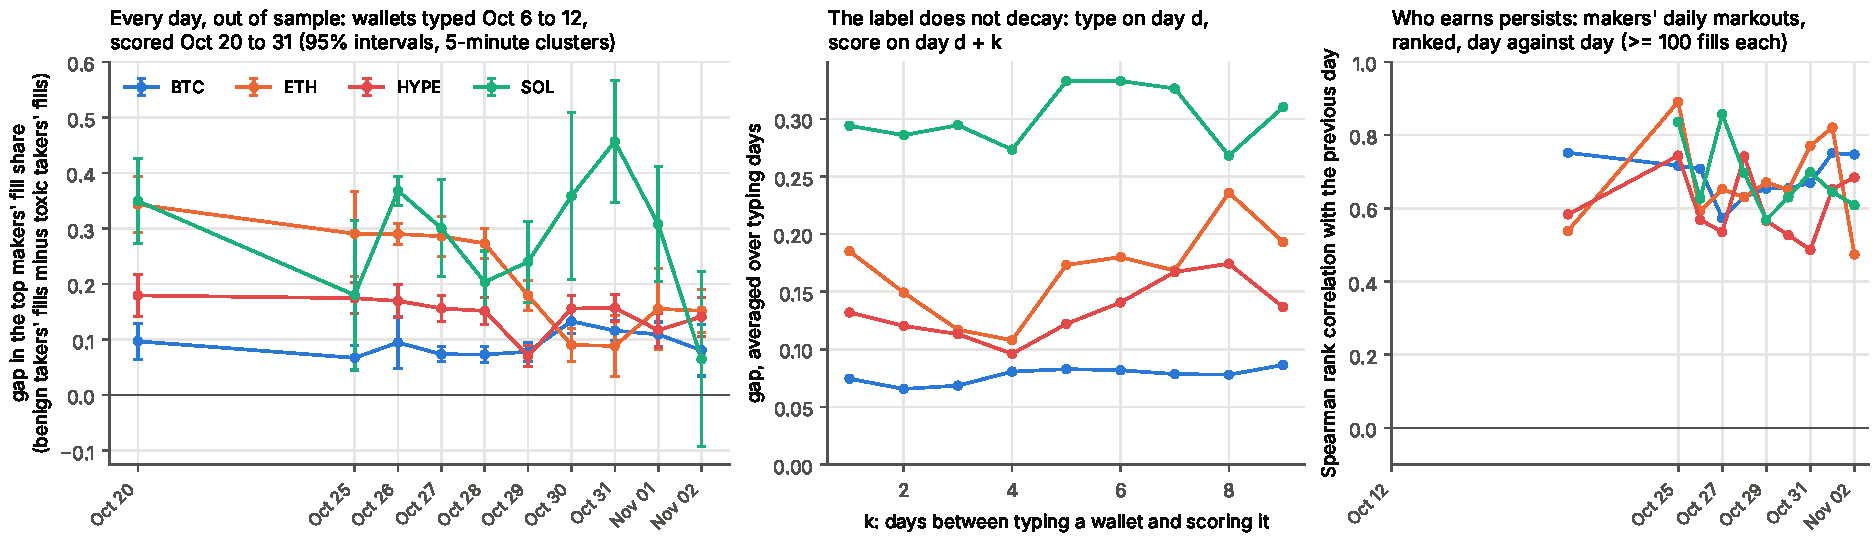
\includegraphics[width=0.9\textwidth]{fig_longwindow.pdf}
\caption{The gap by day, by the distance between typing and scoring, and the persistence of maker rankings.}\label{fig:long}
\end{figure}

\paragraph{A stress episode.} On October 29 a large exchange's wallet was drained and ETH was sold heavily for several hours. On ETH the identity gap failed for five hours: one high-volume, identity-blind wallet among the top ten raised its share of their fills from 3--15\% to 23--39\% and lost $1.4$--$2.3$ bps per fill; without it the other nine's share of toxic fills stayed near its usual level. On BTC, which moved on contagion, the gap held in every hour and the top-10 earned $+0.95$ bps in the first hour. A scheduled announcement the day before, used as a control, was absorbed within one hour. The participant that cannot see who it trades with holds the toxic flow; this is the prediction of the queue model below.

\section{When the price cannot move: the queue game and defences}\label{sec:rq3}

\paragraph{Selection is the whole game.} With the spread pinned at the break-even quote a fill is worth $+0.15$ on average, $+1.10$ in the calm regime and $-2.26$ in the toxic one. An entrant that rests only when its forecast makes the fill worth taking earns $0.14$--$0.16$ per period against incumbents that always rest; its fills are 16\% informed against their 29--31\%, and identity's edge over the anonymous tape grows with the mark lag ($+0.04\to+0.10$).

\paragraph{Learned incumbents.} Tabular Q-learning cannot learn to queue: time priority pays only after several consecutive periods in line, which exploration breaks. Incumbents that run a no-regret rule (EXP3) over complete policies (always rest, never rest, select on the anonymous tape), alongside a \emph{fringe} of always-resting makers, learn to select within a few hundred episodes. Identity is then worth more to the entrant ($+0.05$ to $+0.06$ per period at every lag, five of five seeds), and the fringe's payoff falls from about zero to $-0.02$ to $-0.10$: identity-blind resting liquidity is the counterparty of the selection rent, in the model as on the book.

\paragraph{Steering the queue incumbents.}\prelim{} A no-regret learner can be steered by an opponent that commits to a policy while it learns \cite{dss}, and in the spread mode steering is worth the whole rent. In the queue mode it is worth nothing we can measure. An entrant that always rests while the incumbents learn and switches to identity selection afterwards earns $0.084$ per period against $0.083$ when it was absent during their learning (three seeds, $\rho_z=0.9$). Its presence does change what the incumbents learn (the weight on selecting rises from $0.38$ to $0.68$ when the entrant itself selects), but its own profit moves by $+0.009$, inside the seed noise. The entrant's take in the queue comes from selection against the taker flow, and there is no reaction function to steer.

\paragraph{Venue levers.} \emph{Anonymity.} With a late mark and no identities, incumbents cannot tell a toxic spell in time and keep resting: an uninformed taker is filled 71--75\% of the time in the toxic regime and incumbents earn about zero. With identities they withdraw (fill probability $0.23$--$0.30$; incumbents earn $0.12$--$0.14$) and an identity-blind maker among them earns $-0.13$ to $-0.29$. Anonymity is a transfer from makers to uninformed takers in stress. \emph{Priority fee.} A fee to be served ahead of non-payers turns the queue into an all-pay auction: at the venue's revenue-maximising level it collects two to four times the makers' total rent and leaves every maker at or below zero; a cheap fee doubles the best-informed maker's profit; the fringe pays.

\emph{Request allowance.}\prelim{} Hyperliquid ties the number of orders an address may place to its traded volume. A selector is exactly a maker that cancels and re-places, so we give every maker an allowance of placements per episode, plus one per fill (Figure~\ref{fig:budget}; three seeds). Unconstrained, the identity selector earns $+0.10$ per period more than a maker that simply rests, and the always-resting fringe earns $-0.025$. At an allowance of two placements per hundred periods the selector's edge is $+0.03$; at one it is gone ($-0.015$) and the fringe earns $+0.030$. A tight allowance is the one lever here that removes the selection rent and returns the toxic flow to the makers who were stepping around it. Its cost is depth: selecting makers are locked out of 38--48\% of the periods in which they want to rest. Holding each decision for a minimum time does not help the selector. When regimes are long ($\rho_z=0.99$) selectors rarely change state and the allowance hardly binds.

\begin{figure}[t]\centering
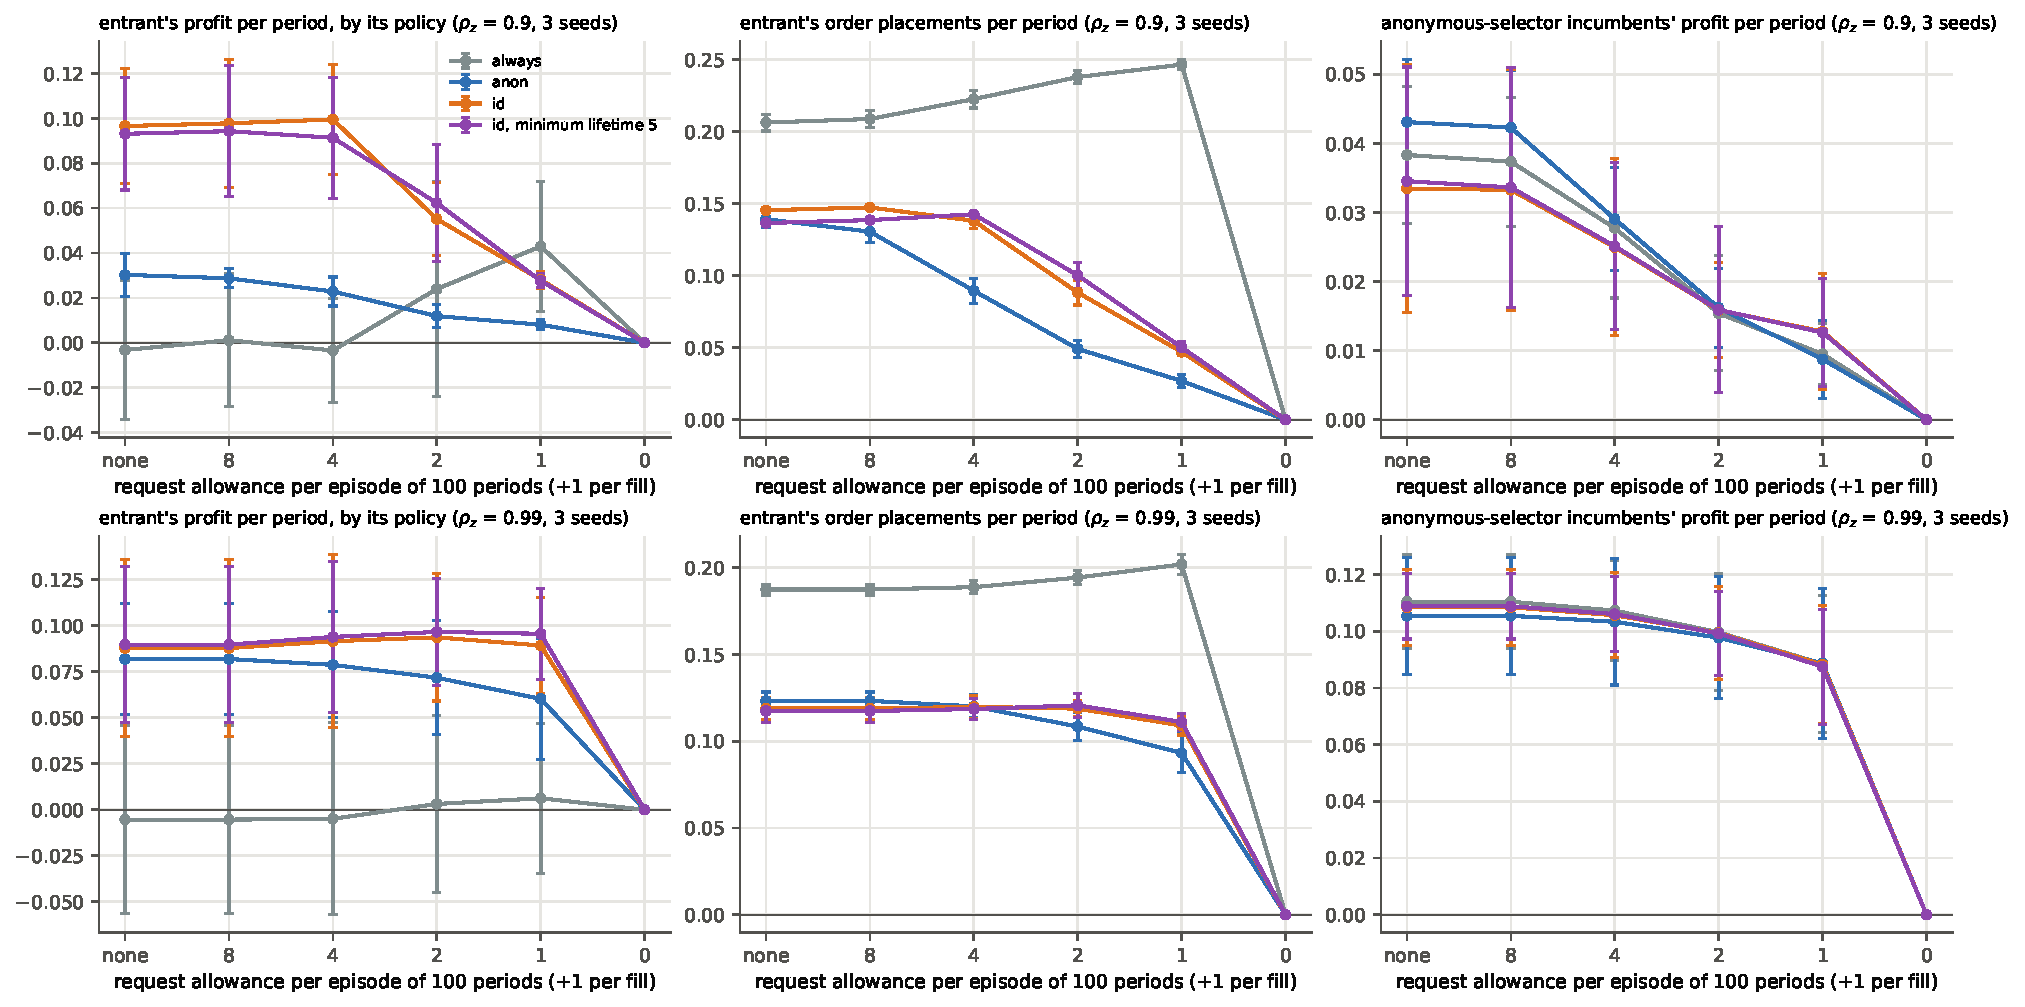
\includegraphics[width=\textwidth]{fig_queue_budget.pdf}
\caption{The request allowance: the entrant's profit by policy, its order placements, and the incumbents' profit.}\label{fig:budget}
\end{figure}

\paragraph{The makers' own levers.} We wrap 20 spread-mode cartels in each of three defences and face them with a set of adversaries. Requoting only every 2--5 periods costs everything against the rule adversaries ($\kappa_A\to1.0$--$1.3$). Randomising the quote costs profit and buys nothing. Never quoting inside the break-even of the identity-based toxicity forecast is the only lever that raises both profit alone and profit under attack by the rule adversaries, and only where the toxic regime bites ($\bar\alpha=0.5$: worst case $0.08\to0.19$).

\paragraph{One frontier.}\prelim{} Figure~\ref{fig:frontier} places every lever on the same two axes: what the incumbents earn with no attack and what they earn against the worst attacker in our set. In the spread mode the rule adversaries leave a defended cartel part of its rent; the exact best response and the public-information attacker, which estimates a randomised reaction function by the most frequent answer, are being added to this comparison (\texttt{slurm/workshop2.sh}, step 5), and on the first cartel they leave it nothing under every defence tested. In the queue mode the levers move incumbents along the diagonal: what they lose to the worst entrant is what the lever took from everyone.

\begin{figure}[t]\centering
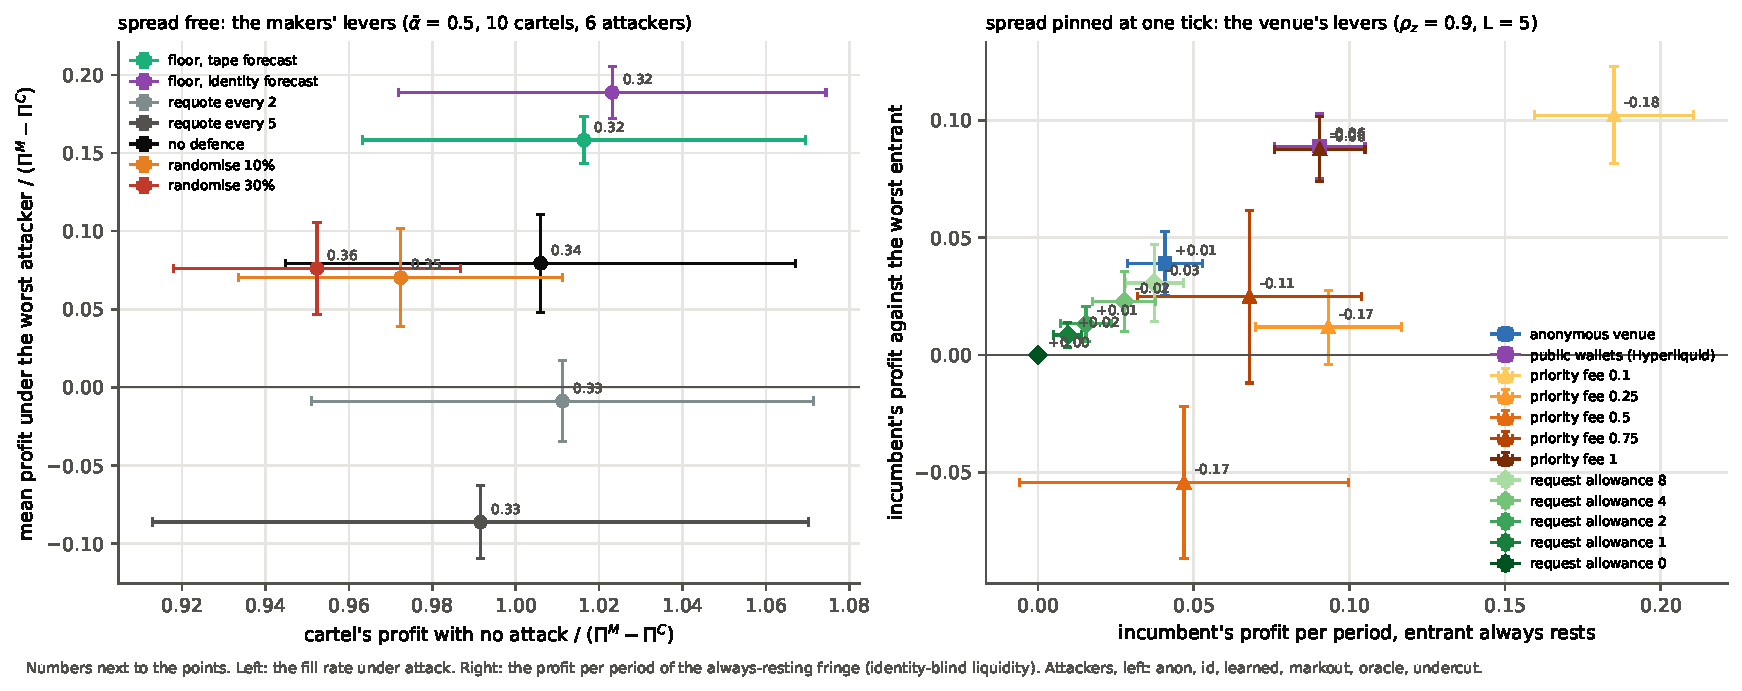
\includegraphics[width=\textwidth]{fig_frontier.pdf}
\caption{Profit alone against profit under the worst attacker, for the makers' levers (left, spread mode) and the venue's levers (right, queue mode).}\label{fig:frontier}
\end{figure}

\section{Discussion and limitations}

\paragraph{What the results say together.} The learners' memory is what creates the rent and what exposes it: a policy that conditions on the last quotes is a reaction function, a reaction function on a public book is identifiable, and an identified reaction function is solvable. Against that attacker neither continued learning nor the makers' own defences protect the rent. What the venue controls is the distribution of the toxic flow, through what makers may know about who is trading and through how places in the queue are allocated.

\paragraph{Limitations.} Takers are stylised: one unit per period, two types, a two-state regime. The value is redrawn each period, so there is no inventory risk and no price discovery. Incumbents are tabular learners with a two-variable state; function-approximation learners may be harder to identify and are untested. The exact best response and the public attacker assume the entrant's own fills do not change the taker flow. The one-tick finding is specific to a venue with a five-significant-figure grid on high-priced assets. The data cover four coins over four weeks on one venue; wallet types need at least 30 fills, so only active takers are typed; a faster price feed from another venue is not excluded as part of the top makers' signal on fills that precede a price move, though it cannot produce the gap on fills that do not. Depth beyond the best price, where the data place most of the taker's cost, is not modelled.

\paragraph{Reproducibility.} Code, tests, summary results and the commands that produce every number are at \url{https://github.com/pradeepu191/wargame}; \texttt{make figures} regenerates the figures from the committed summaries, and a browser replay of the simulator (\texttt{demo/index.html}) shows each experiment period by period.

\appendix
\renewcommand{\thesection}{\Alph{section}}
\section{Complete definitions}\label{app:glossary}
\let\oldsection\section
\renewcommand{\section}[1]{}  % glossary.tex opens with its own \section; this appendix already has one
% Definitions and notation.  \input this section before the model in any document for a
% games / control / security reader; every microstructure term is defined here once, in that
% vocabulary, and then used freely.  Standalone build: paper/glossary_standalone.tex.
\section{Definitions and notation}\label{sec:defs}

This project is a security game played on a financial market, and most of its vocabulary comes
from market microstructure. Each term below is defined once, in the language of games and
control, and then used without further comment. The cast first; then the one-period interaction;
then the benchmarks, the adversary, information, the pinned-spread mode, and the quantities we
measure on real data.

\subsection*{The cast}
\begin{center}\small
\begin{tabular}{p{0.21\linewidth}p{0.74\linewidth}}
\toprule
\textbf{Role} & \textbf{Who it is, and what it chooses} \\
\midrule
Venue (designer) & Sets the rules of the game: the action grid (tick size), what is public (anonymity), and how ties among agents playing the same action are allocated (priority). Hyperliquid in the data; a parameter set in the simulator. \\
\addlinespace
Market makers, incumbents (defenders) & $N$ agents who each period post a standing offer to trade at a price and are paid when another agent accepts it. They learn from their own reward (tabular Q-learning) and, once trained, are frozen and evaluated. \\
\addlinespace
Takers (nature) & One short-lived agent per period who accepts a standing offer or not. With probability $\alpha$ she is \emph{informed}---she knows the state---otherwise she trades for private reasons unrelated to the state. Takers are not strategic: they are the stochastic environment, with a hidden Markov state (the regime) that governs how often the informed type arrives. \\
\addlinespace
Entrant, attacker (adversary) & One additional maker added to a trained population, playing a best response. What it is allowed to observe (its information set) is the treatment variable; what it does to the incumbents' payoff is the exploitability statistic. \\
\bottomrule
\end{tabular}
\end{center}

\subsection*{A. The one-period interaction}
\begin{description}
\item[Mid $m_t$.] The public reference price at the start of period $t$. The state everyone sees.
\item[Fundamental $V_t$.] The true value, $V_t=m_t\pm d$ with $d\sim\mathrm{Exp}(\mu)$, redrawn each period. The state only the informed taker sees.
\item[Quote, half-spread $h$ (the action).] A maker's standing offer: sell at $m_t+h\theta$, buy at $m_t-h\theta$, with $h\in\{1,\dots,K\}$. Symmetric by assumption. The \emph{spread} is $2h\theta$.
\item[Tick $\theta$.] The discretisation of the action space: the smallest price increment. On Hyperliquid, prices carry five significant figures, so one tick is \$1 on BTC near \$80{,}000 and \$0.001 on a \$90 coin.
\item[Best quote, inside, touch.] The lowest half-spread among the makers; \emph{at the touch} means at that price. The taker always hits the best quote; ties are split uniformly (or by priority, below).
\item[Fill, print, trade.] An accepted offer. The \emph{print} is its public record: price, size, side, and on Hyperliquid the wallet on each side.
\item[Informed fill, adverse selection, toxic flow.] A maker's payoff on a fill is $p-V_t$ on a sale and $V_t-p$ on a purchase. The informed taker accepts only when that is negative for the maker, and with the exponential edge an informed fill costs the maker exactly $\mu$ in expectation at every $h$ (memorylessness). \emph{Adverse selection} is this expected loss from being matched with the informed type; \emph{toxic flow} is order flow with a high informed share; a \emph{toxic wallet} is one whose orders are informed with high probability.
\item[Payoff function $\Pi(h;\alpha)$.] A maker's expected one-period payoff from quoting $h$ when it holds the best quote, with $x=h\theta$:
\[
\Pi(h;\alpha)=(1-\alpha)\,2x\,\bar\Phi(x/\sigma_L)\;-\;\alpha\,\mu\,e^{-x/\mu},
\]
the uninformed taker's acceptance probability times the margin, minus the informed type's probability of arriving and accepting times $\mu$. Linear in $\alpha$; closed form.
\end{description}

\subsection*{B. Benchmarks: the Nash point and the cartel point}
\begin{description}
\item[Competitive half-spread $h^C$.] The smallest grid point with $\Pi(h;\alpha)\ge0$: the zero-profit action. It is the Nash equilibrium of the one-shot pricing game---at any $h>h^C$ a maker gains by moving to $h-1$ and taking the whole flow---and the Bertrand outcome of price competition on a grid.
\item[Monopoly half-spread $h^M$.] $\arg\max_h\Pi(h;\alpha)$: the joint payoff-maximising action, what a single maker or a perfectly coordinated group would play. $\Pi^C,\Pi^M$ are the payoffs at $h^C,h^M$.
\item[Rent.] Payoff above the Nash benchmark, $\bar\Pi-\Pi^C$. \emph{Rent units} are $\Pi^M-\Pi^C$, the rent available; dividing by them makes $\alpha$ and $N$ comparable.
\item[Collusion index $\Delta$, rent index $C(\pi)$.] $(\bar\Pi-\Pi^C)/(\Pi^M-\Pi^C)\in[0,1]$: where the population sits between the Nash point (0) and the joint-monopoly point (1). $\Delta$ is the quantity for a learning population \cite{calvano}; $C(\pi)$ the same quantity for a frozen policy profile $\pi$ under evaluation.
\item[Cartel, tacit collusion.] A profile with $C>0$ sustained by independent learners that never communicate: a payoff-dominant profile that is not a one-shot equilibrium, held up in the repeated game by the learned policies' reactions to deviations.
\item[Undercutting.] The deviation to $h-1$ when a rival is above $h^C$: a slightly smaller margin on the whole flow instead of a share of it. The myopic best response, and the quantity that decides whether a profile is a one-shot equilibrium.
\item[Restraint (the mechanism test).] In states where a rival quotes at or inside $h^M$, whether the learner's greedy action is the undercut or not. Reported as the share of such states in which the learner forgoes the undercut, the one-period reward it forgoes, and the Q-value gap. Restraint distinguishes learned coordination from failure to explore.
\end{description}

\subsection*{C. The adversary and exploitability}
\begin{description}
\item[Frozen population $\pi$.] The incumbents' learned policies with learning switched off. The object being attacked.
\item[Nominal payoff $\Pi_{\mathrm{nominal}}(\pi)$.] The incumbents' payoff alone. With an attacker $A$ in the game their payoff is $J(\pi;A)$.
\item[Best-response loss $L_{\mathrm{BR}}$.] $L^A_{\mathrm{BR}}(\pi)=\Pi_{\mathrm{nominal}}(\pi)-J(\pi;A)$ and $L_{\mathrm{BR}}=\max_A L^A_{\mathrm{BR}}$: how much the adversary costs the defenders. The game is general-sum, so the defenders' loss---not the attacker's gain---is the exploitability statistic.
\item[Fraction of rent destroyed $\kappa_A$.] $L^A_{\mathrm{BR}}/(\Pi_{\mathrm{nominal}}-\Pi^C)$. $\kappa_A=1$ means the attacker drives the defenders back to the Nash point.
\item[Attacker types.] The \emph{one-tick undercutter} (quotes one tick inside the best incumbent); the \emph{markout entrant} (a profit-maximising best responder that learns from its own fills' realized payoffs); the \emph{damage-maximising attacker} (minimises $J$ rather than maximising its own payoff; the worst case); the \emph{steering attacker} (targets the incumbents' reaction function rather than their quote: the exact best response, which gives up a little profit today to keep the cartel wide tomorrow). Held-out attackers: $\mathcal{A}_{\mathrm{train}}\cap\mathcal{A}_{\mathrm{test}}\approx\emptyset$.
\end{description}

\subsection*{D. Information}
\begin{description}
\item[Information set $\mathcal{F}$.] What a policy may condition on. Three nested observation models for the entrant: $\Fanon$ (the public tape and book only) $\subset\Fid$ (plus the wallet identity on every print) $\subset\For$ (plus the hidden state). An upper bound and two implementable policies.
\item[Wallet, identity.] The persistent public pseudonym on every order and print on Hyperliquid. Not a name; a label that is the same tomorrow.
\item[Taker type $\alpha_j$.] Wallet $j$'s probability of being informed on any given order. In the simulator, $M$ wallets with types taken as stratified quantiles of $\mathrm{Beta}(\bar\alpha\kappa_\alpha,(1-\bar\alpha)\kappa_\alpha)$: the mean is pinned at $\bar\alpha$ and the concentration $\kappa_\alpha$ sets the dispersion ($\kappa_\alpha\to\infty$ is the homogeneous model).\footnote{Earlier drafts wrote the concentration as $\kappa$, which collides with the fraction of rent destroyed $\kappa_A$. The concentration is $\kappa_\alpha$ from here on.}
\item[Regime $z_t$.] A hidden Markov state, $z_t\in\{\text{calm},\text{toxic}\}$, kept with probability $\rho_z$ per period and otherwise redrawn. In the toxic state the informed-heavy wallets are the active ones. From the entrant's side this is a partially observed Markov decision process; its policy carries a belief over $z_t$.
\item[Mark lag $L$.] The number of arrivals before a print's realized payoff (its \emph{mark}) becomes public. The delay before the state is revealed. $L=0$ would mean the tape tells you immediately who was informed; the data say $L$ is several arrivals.
\item[Regime filter, $\alpha_{\mathrm{next}}$.] The entrant's Bayesian posterior over $z_t$ given what its information set shows, and the implied probability that the \emph{next} taker is informed. The quoting rule acts on $\alpha_{\mathrm{next}}$.
\item[Value of identity.] $\pi^{\mathrm{id}}-\pi^{\mathrm{anon}}$: the entrant's payoff gain from seeing wallets. Read from the venue's side it is the cost to the defenders of de-anonymisation, so \emph{anonymity} is a venue lever and this difference is its price.
\end{description}

\subsection*{E. The pinned-spread mode (one-tick books)}
\begin{description}
\item[One-tick book.] A market whose best quotes are one tick apart essentially all the time (BTC, ETH and SOL on Hyperliquid). The action $h$ is then degenerate: nobody can undercut. The same environment with the spread fixed is the \emph{queue game}.
\item[Rest, out.] The binary action at a fixed spread: keep a standing offer at the touch, or withdraw it.
\item[Queue priority (FIFO).] The venue's allocation rule among agents playing the same action: the earliest standing offer is filled first; a maker that withdraws and returns joins the back of the line. Time priority turns ``when to be present'' into the strategic variable.
\item[Priority fee (priced priority).] Paying the venue to be allocated ahead of the queue. A venue lever; the price of position.
\item[Fill value.] $(1-q)\,x-q\,\mu$: the expected payoff of a fill at half-spread $h$ against a taker of type $\alpha$, where $q$ is the probability the fill was informed given that it happened. At the population break-even it is zero on average, positive in the calm regime and negative in the toxic one. \emph{Selection} is choosing which fills to accept; on a one-tick book it is the only source of payoff above zero.
\item[Selection cartel.] Makers who leave the toxic flow to each other---the analogue, when the spread cannot move, of a cartel that holds the spread above $h^C$.
\item[Depth; sweep, walk.] Depth is the quantity standing at each price. An order larger than the quantity at the touch is filled at successively worse prices: it \emph{walks} the book (a \emph{sweep}). The makers it reaches were standing behind the inside.
\end{description}

\subsection*{F. What we measure on real data}
\begin{description}
\item[Basis point (bp).] $10^{-4}$ of the price. All payoffs on real data are in basis points of the fill price.
\item[Maker and taker side.] On every print one wallet had the standing offer (the maker, the defender's role) and one accepted it (the taker, the aggressor).
\item[Markout at $\tau$.] The maker's ex-post payoff on one fill, scored against the mid $\tau$ seconds later: $-s\,(m_{t+\tau}-p)/p\times10^4$ with $s=+1$ if the maker sold. It includes the half-spread earned at the fill; negative means the fill lost money by $\tau$. The simulator's per-fill reward is the same object with $V_t$ in place of $m_{t+\tau}$.
\item[Effective spread.] $2s\,(p-m_t)/p\times10^4$ with $m_t$ the mid of the last book \emph{before} the fill: what the taker paid relative to the price she could see. On a one-tick book a fill at the touch has effective spread exactly one tick.
\item[Realized spread at $\tau$; price impact.] $2s\,(p-m_{t+\tau})/p\times10^4$ is what the maker kept after $\tau$; the difference, effective minus realized, is the \emph{price impact}: how far the mid moved in the taker's direction. Permanent impact is information; transient impact is liquidity (the price reverts).
\item[Trade-price proxy, bid--ask bounce.] Using the next trade price in place of the mid overstates the maker's payoff because consecutive prints alternate between the bid and the ask. All markouts in this document use the true mid from the recorded book.
\item[Conditional markout; identity given the anonymous signal.] The next fill's markout conditioned on whether the previous taker was a toxic wallet (the identity signal), and the same conditioned additionally on whether the price has already moved against the previous maker (what an anonymous quoter can see). The second isolates what identity adds beyond the tape.
\item[Market-maker wallet.] A wallet with maker share $\ge0.7$ and both buys and sells (two-sidedness $\ge0.3$) over the window. The classification uses activity only, never the outcome being measured.
\end{description}

\subsection*{G. Planning vocabulary (Lecture 15, ``Planning with a Model'')}
\begin{description}
\item[Markov decision problem (MDP).] A state set $X$, an action set $A$, transition probabilities $P(x'\mid x,a)$, an expected one-period reward $r(x,a)$, and a discount factor or a turn limit. The decision maker sees the state, acts, is paid, and moves to the next state. Against a \emph{frozen} cartel the entrant faces an MDP: the state is last period's quotes, the action is its own quote, and $P$ is the cartel's reaction function (deterministic). The cartel is part of $P$, as a target that does not respond to the policy is.
\item[Valid state.] A summary of the history that, with the chosen action, predicts the next reward and the next state as well as the whole history would. The cartel's learners condition on their own last quote and the best rival quote, so last period's quote vector is a valid state for the entrant.
\item[Policy; myopic policy.] A rule that picks an action in each state. The \emph{myopic} policy picks the action with the highest reward today (discount $0$) and ignores the state it leaves.
\item[Bellman equation; backward induction; value iteration.] The optimal value from a state is the best, over actions, of today's reward plus the value of the state that follows. With a turn limit it is solved exactly by working back from the last period (\emph{backward induction}); with a discount, by repeating that step until the values stop changing (\emph{value iteration}). Our exact best response is backward induction over a 100-period episode.
\item[Model-based, model-free.] A model-based decision maker computes its policy from $r$ and $P$; a model-free one learns action values from experience without them. The exact best response is model-based with the true $P$; the public-information attacker is model-based with an estimate of $P$ built from the public book; the cartel's Q-learners are model-free.
\item[Belief state.] When part of the state is hidden, the decision maker's posterior over it, here as counts of outcomes, used as the state. For an identity-aware maker, the per-wallet record of fills and toxic fills plays this role.
\item[Selective feedback; trap.] Some actions reveal nothing about the unknown (a maker that stops trading with a wallet sees no more of that wallet's fills). A policy can then stop on the worse action for ever, even when it is optimal under the decision maker's own beliefs (Rothschild, 1974).
\item[Ordinary trader.] The participant with the least information. A \emph{customer who has to trade} is the model's uninformed taker; her \emph{gains from trade} are her private reason to trade minus the half-spread, in closed form. A \emph{speculator} bets on the direction of the price without information; she does not know $p$, her probability of being right, and her belief after $n$ bets with $k$ right is the belief state $(n,k)$.
\item[Hurdle $p^*$.] The probability of being right that a directional market order needs to break even: $p^*=\tfrac12+x/(2\mu)$, with $x$ the half-spread and $\mu$ the mean size of a price move. Above one, no directional bet can pay.
\item[Quitting line; ruin.] The number of wrong calls after $n$ bets at which the speculator's optimal policy stops for good. \emph{Ruin} is losing all the savings she set aside.
\item[Player, not part of $P$.] An opponent that responds to the policy (a cartel that keeps learning) cannot be folded into $P$. The problem is then a game.
\end{description}

\subsection*{H. Rigour vocabulary}
\begin{description}
\item[Seed intervals.] Every simulator number is a mean over independent training seeds with a 95\% interval; policies compared under common random numbers.
\item[$\mathrm{CVaR}_{0.05}$.] The mean of the worst 5\% of outcomes; reported with the mean so ``robust'' cannot mean ``withdrew''.
\item[Train at $\alpha$, test at $\alpha'$.] Policies trained in one environment and evaluated in another, to separate learned structure from overfitting.
\item[Chronological split.] On data, wallet classification on the first half of the window, measurement on the second.
\end{description}

\subsection*{Notation}
\begin{center}\small
\begin{tabular}{llp{0.5\linewidth}}
\toprule
Symbol & Name & Meaning \\
\midrule
$\theta,K$ & tick, grid size & action grid $h\in\{1,\dots,K\}$ in ticks \\
$\alpha,\bar\alpha$ & toxicity & probability a taker is informed; population mean \\
$\mu$ & informed edge & mean of the exponential edge $d$; the expected cost of an informed fill \\
$\sigma_L$ & liquidity dispersion & s.d. of the uninformed taker's private valuation \\
$\Pi(h;\alpha)$ & payoff function & expected one-period payoff of quoting $h$ \\
$h^C,h^M$; $\Pi^C,\Pi^M$ & Nash, monopoly & competitive and joint-monopoly actions and payoffs \\
$\Delta$, $C(\pi)$ & rent index & $(\bar\Pi-\Pi^C)/(\Pi^M-\Pi^C)$ for a learning / frozen population \\
$L_{\mathrm{BR}}$, $\kappa_A$ & exploitability & defenders' loss against attacker $A$; fraction of rent destroyed \\
$\Fanon\subset\Fid\subset\For$ & information sets & tape and book; plus wallets; plus the hidden state \\
$\alpha_j$, $\kappa_\alpha$ & wallet types & wallet $j$'s informed probability; concentration of the type distribution \\
$z_t$, $\rho_z$ & regime & hidden calm/toxic state and its persistence \\
$L$ & mark lag & arrivals before a print's realized payoff is public \\
$\alpha_{\mathrm{next}}$ & forecast & entrant's posterior probability that the next taker is informed \\
$q$ & fill-conditional toxicity & $P(\text{informed}\mid\text{fill at }h)$ \\
$p$, $m_t$, $m_{t+\tau}$, $s$ & on data & fill price, pre-trade mid, mid $\tau$ s later, $+1$ if the maker sold \\
\bottomrule
\end{tabular}
\end{center}

\let\section\oldsection

\begin{thebibliography}{99}\small
\bibitem{as} M. Avellaneda, S. Stoikov. High-frequency trading in a limit order book. \emph{Quantitative Finance} 8(3), 2008.
\bibitem{gm} L. R. Glosten, P. R. Milgrom. Bid, ask and transaction prices in a specialist market with heterogeneously informed traders. \emph{J.\ Financial Economics} 14, 1985.
\bibitem{calvano} E. Calvano, G. Calzolari, V. Denicol\`o, S. Pastorello. Artificial Intelligence, Algorithmic Pricing, and Collusion. \emph{AER} 110(10), 2020.
\bibitem{cfl} J.-E. Colliard, T. Foucault, S. Lovo. Algorithmic Pricing and Liquidity in Securities Markets. \emph{Review of Financial Studies}, 2026.
\bibitem{cont} R. Cont, W. Xiong. Dynamics of market making algorithms in dealer markets: learning and tacit collusion. \emph{Mathematical Finance} 34(2), 2024.
\bibitem{ccp} \'A. Cartea, P. Chang, J. Penalva. Algorithms and Supracompetitive Prices in Electronic Markets: The Impact of Tick Size. SSRN 4105954, 2026.
\bibitem{dgj} W. W. Dou, I. Goldstein, Y. Ji. AI-Powered Trading, Algorithmic Collusion, and Price Efficiency. NBER WP 34054, 2025.
\bibitem{dss} Y. Deng, J. Schneider, B. Sivan. Strategizing against No-Regret Learners. \emph{NeurIPS} 2019.
\bibitem{brownmackay} Z. Y. Brown, A. MacKay. Competition in Pricing Algorithms. \emph{AEJ: Microeconomics} 15(2), 2023.
\bibitem{gleave} A. Gleave, M. Dennis, C. Wild, N. Kant, S. Levine, S. Russell. Adversarial Policies: Attacking Deep Reinforcement Learning. \emph{ICLR} 2020.
\bibitem{mcmahan} H. B. McMahan, G. J. Gordon, A. Blum. Planning in the Presence of Cost Functions Controlled by an Adversary. \emph{ICML} 2003.
\bibitem{psro} M. Lanctot et al. A Unified Game-Theoretic Approach to Multiagent Reinforcement Learning. \emph{NeurIPS} 2017.
\bibitem{zhai} D. Zhai. Public Trader Identity: Adverse Selection and Return Predictability. arXiv:2608.04373, 2026.
\bibitem{albers} J. Albers, M. Cucuringu, S. Howison, A. Y. Shestopaloff. An Open Book: Level 4 Order Book Data from the Hyperliquid Exchange. SSRN 6465720, 2026.
\bibitem{hldocs} Hyperliquid Documentation. \url{https://hyperliquid.gitbook.io/hyperliquid-docs}, accessed Oct.\ 2026.
\end{thebibliography}
\end{document}
